\makeheading{中国科学家首次尝试用CRISPR治疗HIV感染

\large{Chinese Scientists use gene-edited stem cells to treat HIV — \ with mixed success}}
\begin{multicols}{2}

研究人员首次尝试使用CRISPR基因编辑技术治疗艾滋病病毒(HIV)感染患者。

For the first time, researchers have used CRISPR gene-editing technology to try to treat a person infected with HIV.

\begin{figure}[H]
\centering
\includegraphics[width=0.5\linewidth]{IMG/201909/190901}
\caption{\textit{艾滋病病毒通过攻击免疫细胞破坏机体抵抗力}}
\end{figure}

\qiangdiao{中国科学家对人类干细胞进行基因编辑,使其天然能够抵御HIV并将其移植到一名罹患血液系统肿瘤的HIV感染者身上。}经基因编辑的细胞在患者体内持续存活了一年多且未引起明显副作用,但细胞数量较少,不足以降低血液中HIV的病毒载量。
\qiangdiao{Scientists in China engineered human stem cells to mimic a rare form of natural immunity to the virus and transplanted them into a man with HIV and blood cancer.} The gene-edited cells survived in the man’s body for more than a year without causing detectable side effects, but the number of cells was not high enough to significantly reduce the amount of HIV in his blood.

“这是在使用基因编辑技术治疗人类疾病道路上迈出的重要一步,”加州大学伯克利分校的生物学家Fyodor Urnov说,“因为这项研究,我们知道了这些\qiangdiao{经编辑的细胞可以在患者体内存活,而且是长时间存活。}”

“This is an important step towards using gene editing to treat human disease,” says Fyodor Urnov, a biologist at the University of California, Berkeley. “Because of this study, we now know that \qiangdiao{these edited cells can survive in a patient, and they will stay there.}”

论文主要作者、北京大学生物学家邓宏魁教授表示,这项研究的灵感来自于十多年前一则骨髓移植似乎治愈了HIV感染的病例报道。

Lead author Hongkui Deng, a biologist at Peking University in Beijing, says that the research was inspired by a remarkable bone-marrow transplant that seemingly cured a man of HIV more than a decade ago.

\section*{突变带来的希望 Mutant power}

2007年,最初被称为“柏林病人”的Timothy Ray Brown因为白血病接受了骨髓移植。但骨髓供体非常特殊,携带了特别版本的\textit{CCR5}基因,对HIV具有免疫力。

In 2007, Timothy Ray Brown ― initially known as ‘the Berlin patient’ ― underwent a bone-marrow transplant to treat his leukaemia. The bone-marrow donor was special, however, in that he had a version of the \textit{CCR5} gene that confers immunity to HIV.

通常情况下,\textit{CCR5}基因编码的是白细胞上的一种受体,HIV病毒主要通过该受体进入细胞。如果个体携带两个\textit{CCR5}突变拷贝,这种受体会发生弯曲并阻止某些HIV病毒株进入细胞。但这种抗HIV基因特别罕见:仅在1\%的欧洲血统人口中有发现,在其他种族群体中几乎不存在。

Normally, the gene encodes a receptor on the surface of white blood cells that the HIV virus uses to infiltrate cells. But in people with two copies of the \textit{CCR5} mutation, this receptor is warped and blocks certain strains of HIV from entering cells. The HIV-resistant version of the gene is exceptionally rare: it’s found in just 1\% of people of European descent, and is virtually nonexistent in other ethnic groups.

医生们成功地通过骨髓移植,用对HIV有抵抗力的免疫细胞取代Brown原有的免疫细胞。近13年过去,Brown的血液中未再检测到HIV病毒存在的迹象,白血病则处于持续缓解期。今年3月,研究人员报道第二名患者在英国接受了类似的手术,并被治愈。

Doctors hoped that the bone-marrow transplant would replace Brown’s HIV-susceptible blood cells with immune ones — and it did. After nearly 13 years, there is no sign of HIV in his blood, and his leukaemia is in remission. In March, researchers reported that a second person underwent a similar procedure in Britain and was cured.

邓教授希望通过\qiangdiao{CRISPR基因编辑技术}对来自\qiangdiao{正常供体的血液干细胞}进行基因编辑,使其\qiangdiao{具备HIV抵抗性},进而让这种潜在的治愈方法更具可推广性。他和同事们在一名27岁的中国男性身上对这种方法进行了测试,该男子携带HIV且罹患白血病,需进行骨髓移植手术。他们从供体内提取\qiangdiao{骨髓干细胞},并利用\qiangdiao{CRISPR-Cas9技术}将其转化为\qiangdiao{\textit{CCR5}突变体}。

Deng wanted to use \qiangdiao{CRISPR gene editing} to engineer \qiangdiao{HIV-resistant blood stem cells from normal donors}, making this potential cure more widely accessible. He and his colleagues tested this approach on a 27-year-old man in China who had been diagnosed with HIV and leukaemia, and who needed a bone-marrow transplant. The scientists extracted bone-marrow stem cells from a donor and \qiangdiao{used CRISPR–Cas9 to transform them into \textit{CCR5} mutants.}

最终,研究团队成功对他体内的17.8\%的供体干细胞进行了基因编辑。

Eventually, the were able to edit 17.8\% of the donor’s stem cells.

\section*{安全第一 Safety First}

为最大限度地提高骨髓移植治疗患者白血病的概率,研究人员将经基因编辑的干细胞与原始干细胞进行了混合。研究团队在移植后对该患者进行了持续监测,以了解经基因编辑的细胞能否存活和复制,是否能治愈HIV感染,以及最重要的——治疗是否安全。

To maximize the chance that the transplant would treat the patient’s cancer, the researchers mixed the edited stem cells with unedited ones. The team monitored the man after the transplant to see whether the edited cells would survive and replicate, whether they treated the HIV infection and, most importantly, whether the treatment was safe.

在人体内使用CRISPR基因编辑技术仍然存在争议,有研究表明,在实验室中CRISPR有时可能会造成预料外的基因突变——如果在人体内发生,其后果可能是灾难性的。

CRISPR gene editing in people remains controversial, in part because many researchers worry about its side effects. Studies have shown that CRISPR sometimes creates unwanted mutations in the lab— and the consequences of that happening in a person could be disastrous.

骨髓移植术后19个月,患者体内仍能检测到占经CRISPR编辑的干细胞,尽管它们仅占患者总干细胞的5-8\%。换句话说,略超过一半的基因编辑干细胞在移植后死亡了。此外,尽管该男子的白血病持续缓解,但他体内仍可检测到HIV。

After 19 months, the CRISPR-edited stem cells did persist, although they comprised only 5–8\% of the recipient’s total stem cells. This means that a little over one-half of the edited cells died after they were transplanted. And although the man’s leukaemia is in remission, he is still infected with HIV.

而邓教授最在意的还是经基因编辑的细胞并未对这名男子造成任何不良影响。此外,也未发现任何预料之外的基因突变证据。

To Deng, the most important thing is that the man did not suffer any side effects caused by the gene-edited cells. And when the researchers sequenced the genomes of those cells, they didn’t find evidence of unintended genetic changes.

\section*{更进一步 Pushing Forward}

美国宾夕法尼亚大学的免疫学家Carl June表示,邓教授的研究为探索使用CRISPR基因编辑技术治疗其他血液疾病,如镰状细胞贫血,打开了新的大门。他着重强调此次研究遵循了严格的伦理规范,包括取得了受试对象的知情同意。

Carl June, an immunologist at the University of Pennsylvania in Philadelphia, says that this proof of concept opens the door for research into testing this technology for treatment of other blood diseases, such as sickle-cell anaemia. He also notes that this study complied with standard ethical protocols, including obtaining informed consent from the participant.

基因编辑技术的进步意味着,研究人员现在可以以高于17.8\%的成功率对干细胞进行编辑;但这也伴随着风险,因为CRISPR每次切割基因组时都有可能发生错误。

Improvements in gene-editing technology mean researchers can now edit stem cells with efficiency greater than the 17.8\% success rate in the latest study. But that comes with risks. Each time CRISPR makes cuts in the genome, there’s a chance something could go wrong. 

这项研究并未取得全面胜利,但它会推动领域向前发展。但现在,研究人员可以用这项研究作为依据,证明这类研究不仅是安全的,甚至还可能带来丰硕的成果。“我今晚要多吃一勺冰淇淋庆祝一下,因为我知道使用基因编辑技术治疗人类疾病,仍在正确的道路上不断向前推进。”Urnov说。

This paper is an incomplete success, but it will only motivate the field to push onwards. Now, he says, researchers can point to this study as proof of concept that this line of research can be safe and potentially fruitful.“I'm going to have an extra scoop of ice cream tonight, knowing that the ship of human genome editing for treating disease is still on course,” says Urnov.

\end{multicols}

\vskip-2em\greybox{\vskip-25pt
\makeheading{生活中的科学}

Q1为什么十五的月亮十六圆?

Q2为什么集装箱的表面都是凹凸不平的?

Q3为什么行星运动的轨道都是椭圆的?

Q4为什么功率较小的电风扇(\textit{例如台式电风扇}),在把插头拔掉后重新按开关还能转1~2圈?是因为具有惯性吗?

}

\vskip-2em\makeheading{地铁列车是怎样调头的}

\begin{multicols}{2}
地铁列车在抵达终点站后,通常会立即调转运行方向往回行驶。地铁列车的“调头”则称为折返。列车的两端均设有司机室,司机只要激活并操作反方向的司机室,即可让列车直接向反方向行驶。

\begin{figure}[H]
\centering
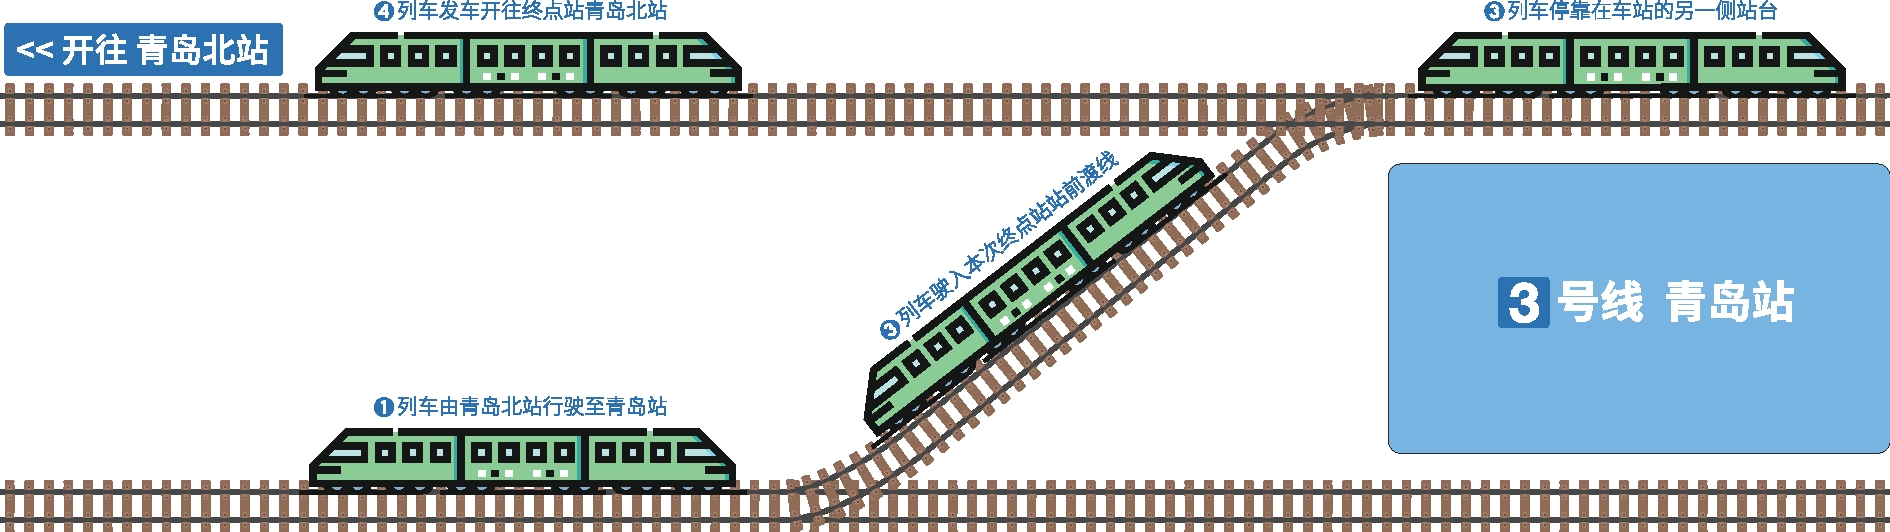
\includegraphics[width=\linewidth]{IMG/201909/BEFORE_SOURCE}
\caption{\textit{地铁3号线在青岛站的站前折返}}
\end{figure}

\qiangdiao{站前折返}指列车利用站前渡线进行折返。以青岛地铁3号线青岛站为例,当列车在抵达青岛站之前,驶入道岔侧向停靠在对面站台,在下客的同时上客,直接改变运行方向驶离。

\begin{figure}[H]
\centering
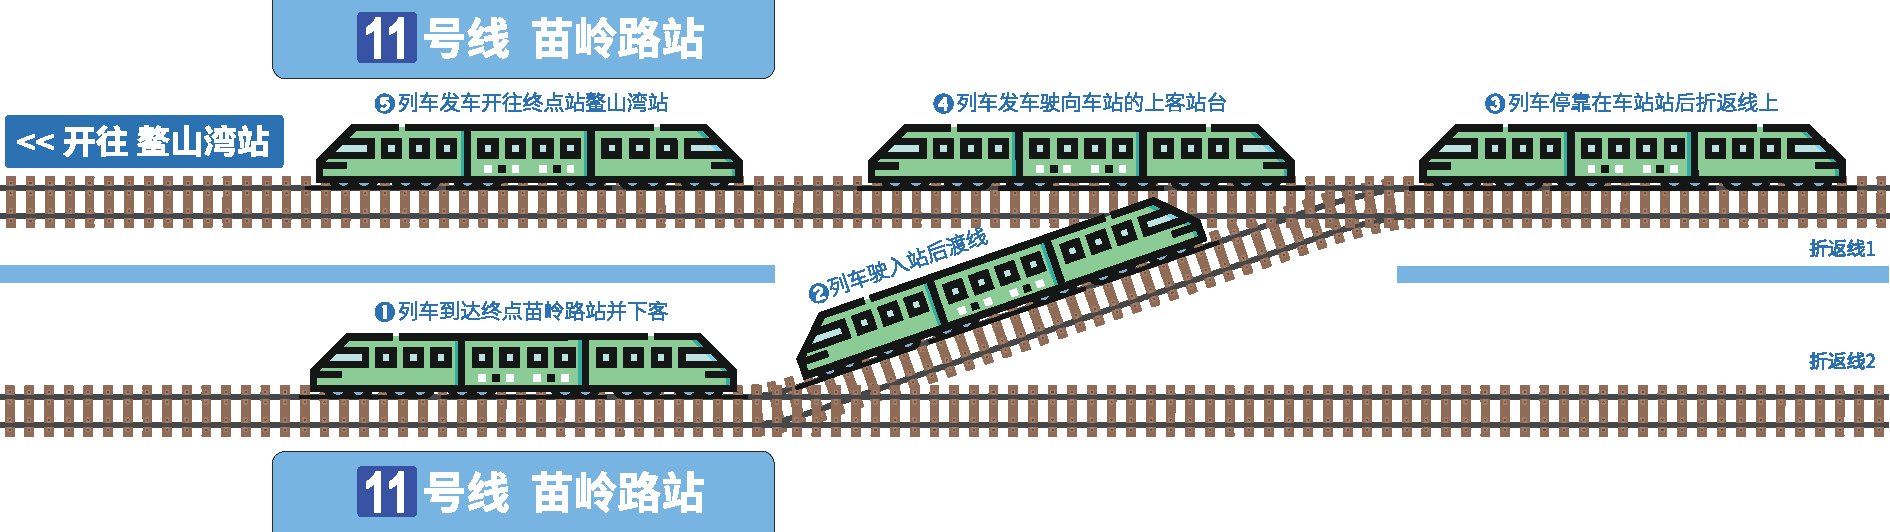
\includegraphics[width=\linewidth]{IMG/201909/AFTER_SOURCE}
\caption{\textit{地铁11号线在苗岭路站的站后折返}}
\end{figure}

\qiangdiao{站后折返}则是列车利用站后渡线进行折返。以青岛地铁11号线苗岭路站为例,列车抵达苗岭路后,先在下客站台清客,清客完毕后继续向前行驶,在站后折返线改变运行方向,驶入上客站台载客。车站站设置了2条站后折返线,列车可在调度指定的任一折返线上进行站后折返。
\end{multicols}

\ADyixuehui

\newpage

\makeheading{食堂阿姨到底能不能准确打出二两饭?}
\begin{multicols}{2}
在同学们看来,食堂阿姨就像“随机数生成器”,打多少饭全看心情。如果要问食堂阿姨如何判断这一勺饭是二两还是三两,多半得到的回答是“凭感觉”。“凭感觉”真的那么准确吗?
\begin{figure}[H]
\centering
\includegraphics[width=\linewidth]{IMG/201909/190902}
\end{figure}


是什么因素决定了我们感知世界的\qiangdiao{“分辨率”}?换言之,我们能够在多大程度上准确区分两个刺激之间的差异?这个过程又是如何进行的?

\section*{测量感知}

几个世纪以来,人们一直认为精神世界与物理世界是完全不同的。尽管无生命物体的运动能够通过数学手段预测,但生命体的行为,长期被认为是在意志的控制下由不同于非生命体的力量驱动的,无法用同样的方式进行预测。

直到 1834 年,德国医生恩斯特·海因里希·韦伯(Ernst Heinrich Weber)要求被试者报告在两个重量差异较小的物体中,他们认为哪一个物体更重。在这些实验中,他发现\qiangdiao{个体做出正确选择的概率只取决于重量间的比率。}

例如,如果一个个体在比较 1 kg和 1.1 kg 的重量时正确率为 75\%,那么该个体在比较 2 kg 和 2.2 kg 的重量时,正确率也为 75\%。或者说,当一个物体的重量是另一个物体重量的 1.1 倍时,该个体的正确识别率为 75\%。

这个简单而明确的规则打开了用数学定律量化人类行为的大门,进而被应用于许多物种的所有感觉模式,这就是众所周知的\qiangdiao{韦伯定律}(\qiangdiao{Weber's Law})。后来韦伯的学生古斯塔夫·费希纳(Gustav Fechner)对这一规律进行了数学描述,因此它也被叫做韦伯-费希纳定律。

\section*{解码韦伯定律}

多年来,研究者们提出了几十个模型,试图解释韦伯定律。虽然它们都可以解释韦伯实验的结果,\qiangdiao{但没有任何实验能够进行验证,找出正确的模型。}

例如,一个十分有影响力的模型就是\qiangdiao{信号检测理论}(\textit{Signal Detection Theory})。信号检测理论认为,人对信号的检测不仅依赖于自身的感受能力,而且依赖于自身所设定的反应标准。在两个人的听觉感受性完全相同的情况下,如果一个人期待着某种声音信号的出现,那他可能会做出较多“信号出现”的判断。

然而理论终归是理论,有许多理论正等待实验的检验。而最近的一项研究发现,学界此前可能忽略了一个关键的变量,那就是\qiangdiao{决策时间}。

一个来自葡萄牙的研究中心的研究团队发现,韦伯定律可以被描述为一个新的心理物理学规则,\qiangdiao{它不仅涉及选择的结果,还涉及做出选择所需的时间。}

在这项新的研究中,Renart 和他的团队训练大鼠区分两种强度略有不同的声音。他们制造了一种专门用于大鼠头部的微型耳机,可以同时向大鼠的两只耳朵传送声音。

在每一次传送到大鼠两只耳朵中的声音中,一边的声音强度会稍微大于另一边,大鼠的任务是通过转向对应的一侧来报告哪边声音更大。我们人类在听到某一边的声音比另一边大时,会自然地看向那一方向“这种行为对大鼠来说是很自然的,因为它们像我们一样,会把头转向声音的来源。”文章的作者之一 Vazquez 解释说。大鼠有足够的时间来听声音,以便做出选择。因此,\qiangdiao{每一次实验尝试都得到了一个选择和一个决策时间。}
\begin{figure}[H]
\centering
\includegraphics[width=\linewidth]{IMG/201909/190903}
\end{figure}

“我们的实验证明,动物的行为符合韦伯定律,”Vazquez 说,“它们分辨两种声音中哪一种声音更大的能力仅仅取决于声音强度的比率。只要两组声音的强度比率相同,大鼠比较两种轻声播放的声音强度的准确性与它比较两种大声播放的声音强度的准确性一样好。 ”这些结论和先前的研究是一致的。

然后,研究团队开始详细分析大鼠需要多长时间来做出决策,后来他们才意识到这是至关重要的一步。他们发现,\qiangdiao{决策时间和两种声音的强度是相互关联的——声音越大,做决策的时间就越短。}例如,在两个声音的相对强度恒定的情况下,区分两种强度较小的声音所用的时间更长,区分两种强度较大的声音所用的时间更短,也就是说,决策时间和音量成反比。

“一般情况下,人们对韦伯定律的研究集中在区分结果的准确性上,这也是韦伯本人所描述的,”Vazquez 解释道,“令人惊讶的是,决策所需的时间很少受到关注。”或许生活中也是如此——和等待时间相比,大家普遍还是更关心食堂阿姨盛的饭份量够不够。

\section*{重塑韦伯定律}

事实上,该研究团队已经发现了一个新的心理物理学定律,他们称之为\qiangdiao{“时间强度等效鉴别”}(\textit{Time-Intensity Equivalence in Discrimination , TIED}),它可以将一对声音的强度和区分它们所需的时间联系起来。该定律不仅与区分的准确性有关,还与所需的时间有关。

为了研究 TIED 是否适用于不同的情境,该研究团队招募人类被试进行了同样的实验,并得到了类似的结果。如果 TIED 的普适性得到验证,这或许能最终帮助学界找出正确的模型。研究团队的分析表明,为了符合 TIED 的规律,解释韦伯定律的数学模型需要满足一系列严格的条件。

接下来,研究团队计划探索他们发现的数学规律如何在大脑中体现。Renart 总结说:“我们想要确定哪些大脑区域在我们的任务中起到重要作用,以及这些回路中的神经元如何对模型中的不同元素执行计算。”

\end{multicols}
\ADhairui
\makeheading{生活中的科学$\cdot$上期答案}
\begin{multicols}{2}
\noindent\qiangdiao{Q1为什么水珠都是圆的?}

\noindent\qiangdiao{A1} 我们都知道,液态水具有很好的流动性。因此,水滴的形状和它所处环境的对称性息息相关。在完全失重的环境中,各个方向都是等价的。因此,水滴在稳定时处于一个各向同性的形状也就是球形。如果水的性质改变,比如结冰,水在失重环境中也不再是球形。如果水滴在下落过程中受到空气阻力,水滴就会变成类似纺锤形。

\noindent\qiangdiao{Q2为什么酒精喷灯的温度高于酒精灯?}

\noindent\qiangdiao{A2} 酒精喷灯的火焰温度高于酒精灯源于酒精喷灯的特殊结构导致的酒精蒸气的相对酒精灯更加充分的燃烧。

通过测量酒精灯的火焰温度,我们可以发现,对于酒精灯而言,其火焰外焰温度高于内焰温度,同时我们发现其外焰温度波动较大,最高可达718℃,最低可达630℃。这是由于外焰长度较长,受环境影响较大;而加了防风罩后的酒精灯火焰外焰温度可达800℃左右且较为稳定,这个温度才是酒精灯外焰可以达到的稳定温度。酒精灯外焰温度比内焰温度高的原因是外焰相比于内焰与空气接触充分,燃烧更加充分,产生热量更多,温度更高。

而对通过测量酒精喷灯的温度,我们会发现其温度基本上都在900℃以上,可高达1063℃,高于酒精灯的火焰温度。这与酒精喷灯的结构设计有关。如

\begin{figure}[H]
\centering
\includegraphics[width=0.4\linewidth]{IMG/201909/190904}\includegraphics[width=0.6\linewidth]{IMG/201909/190905}
\end{figure}

点燃酒精喷灯的过程是往预热盘中注入酒精并将其点燃。等汽化管(预热管或灯芯管)内酒精受热汽化并从喷口喷出时,预热盘内燃着的火焰就会将喷出的酒精蒸气点燃。酒精喷灯中酒精蒸气的燃烧,相比比于酒精灯外焰中更加充分,因此温度更高。

\noindent\qiangdiao{Q3量子纠缠可以瞬时改变量子叠加态,以一定规律测量一组纠缠中的量子,与其纠缠的另一组在很远很远的地方的量子就会有规律的改变量子叠加态,这样可以以摩斯电码的方式传递信息了吗?}

\noindent\qiangdiao{A3} 我们以两个自旋为例子来解答这个问题。我们可以制造两个自旋的纠缠态,在这个状态中一个自旋朝上一个自旋朝下,但是每个自旋即不朝上也不朝下,而是有二分之一的概率朝上二分之一的概率朝下。当你对它们测量时,两个自旋各自塌缩到自旋的本征态上,这时我们会看到一个自旋朝上一个自旋朝下。这种机制看似可以用来传递信息,但是在纠缠态中,我们无法获知自己手里的自旋朝向。因此并不能把自己想要传递的信息有效的传播出去。比如,你想用自旋上来表示"是",但是你不能控制自己手中的自旋向哪个方向塌缩,因此也无法按自己的想法控制对方自旋的朝向,结果就是不能通过这个机制有效传递信息。

\noindent\qiangdiao{Q4光是怎样携带信息的呢?}

\noindent\qiangdiao{A4} 首先,光是一种电磁波,其振幅、频率,相位等物理特性都包含了信息,那么先来简单了解下电磁波是如何作为信息载体进行信号传输的,光携带信息的原理与之类似。

一般的简易通讯模型如图所示,调制器将信源产生的信号加载到载波上,通过无线信道进行传输,然后通过解调器解调,去除噪声后得到信源发出的信息。

\begin{figure}[H]
\centering
\includegraphics[width=\linewidth,clip=true,trim=0 45 0 0]{IMG/201909/190906}
\caption{\textit{简易通信模型}}
\end{figure}

“光怎样携带信息”其实主要是上述模型中的调制过程。由于电磁波具有幅度、频率、相位等特性,那么就可以通过调节电磁波的这三种特性来表现不同的状态,利用这三种特性的调制手段分别称为调幅、调频和调相。

\begin{figure}[H]
\centering
\includegraphics[width=\linewidth,clip=true,trim=0 45 0 0]{IMG/201909/190907}
\caption{\textit{幅度调制示意图}}
\end{figure}

对于模拟信号而言,其幅度调制的原理如图所示。待调制信号幅度随时间变化,频率不确定;在加上一个直流信号后将其幅度抬升到全为正值,然后加载到高频载波信号上,得到调制后的信号具有固定的频率,可以传输的同时其幅度保留着原信号的波形,实现了信息的加载。

从数学上看,一个随时间变化的幅度函数$m’(t)$在经过调制(\textit{假设为正弦波调制})后变为:

\[
[1+m'(t)]\sin (\omega_0t+\phi)
\]


解调器的作用就是根据得到的波形将原信号函数解出来即可,具体解调方式在此不进行介绍。

以上是模拟信号的幅度调制原理,对于数字信号也是如此,其三种调制方式的示意图如下:

\begin{figure}[H]
\centering
\includegraphics[width=\linewidth,clip=true,trim=0 45 0 0]{IMG/201909/190909}
\caption{\textit{三种数字调制方式}}
\end{figure}

数字信号对应0和1的一串字符,转换为电信号可以是电压的开关或者电流的有无,对应的波形是一串矩形波,因此只要在幅度、频率和相位上分别定义两个不同的数值即可进行对应的幅度调制、频率调制和相位调制。如调幅就可以由脉冲波实现。

\end{multicols}

\ADxinhangdao


